\chapter{Datenaugmentierung}
\label{kap:augtheorie}

\section{Begriff, Formalisierung und Wirkmechanismen}
\label{sec:augformal}

Datenaugmentierung bezeichnet die künstliche Vergrößerung eines
Trainingsdatensatzes durch Transformationen, die den semantischen Gehalt der
Beispiele -- und damit ihre Beschriftung -- erhalten \parencite{shorten2019}. Sei
$D = \{(x_i, y_i)\}_{i=1}^{n}$ der Datensatz, $\mathcal{T}$ eine Familie von
Transformationen mit einer Verteilung $p(t)$ und $\tau_t$ die zu $t$ gehörende
\emph{Labeltransformation}. Anstelle des empirischen Risikos minimiert das
Training dann das \emph{augmentierte} Risiko
\begin{equation}
\hat{R}_{\text{aug}}(f) \;=\; \frac{1}{n}\sum_{i=1}^{n}
\mathbb{E}_{t \sim p(t)}\Big[ L\big(f(t(x_i)),\, \tau_t(y_i)\big) \Big],
\label{eq:erm-aug}
\end{equation}
also das Risiko gemittelt über eine \emph{Umgebung} jedes Datenpunkts --
die Vicinal Risk Minimization von \textcite{chapelle2001}.

\absatz{Die Gleichung im Einzelnen.} Weil auf ihr die gesamte Argumentation der
folgenden Kapitel aufbaut, seien die vier Größen benannt, die bei der
Detektion nicht selbsterklärend sind:

\begin{description}[leftmargin=4.2em,style=sameline,itemsep=0pt,
                    font=\normalfont]
  \item[$(x_i, y_i)$] das $i$-te Trainingsbeispiel. Bei der Detektion ist $y_i$
  keine einzelne Zahl, sondern eine \emph{Menge} von Boxen mit Klassenangabe.
  \item[$\mathcal{T}$] die Familie der überhaupt zugelassenen Transformationen --
  die Antwort auf die Frage, \emph{welche} Operationen erlaubt sind. Als eigenes
  Symbol erscheint sie in Gleichung~\eqref{eq:erm-aug} nicht; sie ist die
  \emph{Grundmenge}, über die der Erwartungswert mittelt, denn $p$ ist eine
  Verteilung auf $\mathcal{T}$:
  $\mathbb{E}_{t \sim p(t)}[\,\cdot\,] = \int_{\mathcal{T}}
  (\,\cdot\,)\,\mathrm{d}p(t)$.
  \item[$p(t)$] die Verteilung über $\mathcal{T}$ -- die Antwort auf
  \emph{wie häufig} und \emph{wie stark}. Sie ist das, was die
  Parametertabellen dieser Arbeit dokumentieren.
  \item[$\tau_t$] die zu $t$ gehörende Labeltransformation: wie $y$ verändert
  werden muss, damit es $t(x)$ noch korrekt beschreibt.
\end{description}

Der Unterschied zum gewöhnlichen empirischen Risiko
\[
\hat{R}(f) \;=\; \frac{1}{n}\sum_{i=1}^{n} L\big(f(x_i),\, y_i\big)
\]
liegt allein im Erwartungswert: Statt jedes Beispiel genau in der Form zu sehen,
in der es aufgenommen wurde, sieht das Netz eine ganze Umgebung (die \emph{Vicinity}) davon. Weil
$\mathcal{T}$ überabzählbar ist, wird der Erwartungswert praktisch durch eine
Monte-Carlo-Näherung mit \emph{einer} Ziehung je Bild und Epoche ersetzt. Daraus
folgt eine Konsequenz, die in Abschnitt~\ref{sec:ablation} messbar wird: Starke
Augmentierung und kurzes Training passen nicht zusammen -- der Arm ohne
Verdeckung sättigte dort bereits in Epoche~3, die beiden augmentierten
verbesserten sich bis zur letzten Epoche.

\absatz{Was in dieser Arbeit \emph{ein} $t$ ist.} Keine einzelne Operation,
sondern ein Parametervektor über alle Stufen der Pipeline -- etwa
\enquote{Hintergrund 3, Zoom 1,42, horizontal gespiegelt, Objektrotation
$137^\circ$, Achsverhältnis 0,81, Helligkeit $\times 0{,}92$, Gamma 1,08,
Rauschangleich $\sigma = 4{,}1$, Schlagschatten, JPEG-Qualität 71}. Die
Verteilung $p(t)$ faktorisiert dabei über die einzelnen Transformationen: Die
Anteile der Parametertabelle sind unabhängige Ziehungen. Zwei Ausnahmen sind
bewusst gesetzt und folgen aus Anforderung~A3 -- Objektgröße und
Hintergrundzoom sind gekoppelt (Gleichung~\eqref{eq:zoom}), und die Größen aller
Instanzen eines Clusters hängen an einer gemeinsamen Basisgröße. Eine
unabhängige Ziehung wäre dort physikalisch unmöglich.


Für den vorliegenden Fall lohnt eine letzte Lesart. Weil die Trainingsdaten
nicht erweitert, sondern \emph{erzeugt} werden, ist $n$ winzig -- als
Ausgangsmenge lassen sich die neun Objektausschnitte und sieben Hintergründe
lesen, und $t$ ist der gesamte Generatordurchlauf. Die 6000 Trainingsbilder sind
dann 6000 Ziehungen aus $p(t)$. Die gesamte Vielfalt des Datensatzes steckt
damit in $p(t)$ und in keinem einzigen aufgenommenen Bild -- weshalb die
Dokumentation von $p(t)$ in dieser Arbeit die Dokumentation des Datensatzes
\emph{ist}.

\absatz{Die Labeltransformation ist der kritische Teil.} Neben $t$ tritt in
Gleichung~\eqref{eq:erm-aug} stets $\tau_t$ auf. Bei der Klassifikation ist
$\tau_t = \mathrm{id}$ -- eine gespiegelte Katze bleibt eine Katze --, weshalb
Augmentierung dort begrifflich mit \enquote{label-erhaltend} gleichgesetzt wird.
Bei der Objektdetektion ist $\tau_t \neq \mathrm{id}$: Boxkoordinaten müssen
mittransformiert werden. Ist $\tau_t$ nur \emph{näherungsweise} bekannt, so
entsteht Rauschen im Zielsignal -- genau die in
Abschnitt~\ref{sec:augdetektion} behandelte Fehlerquelle, und der Grund für die
Arbeitsteilung zwischen Generator und Trainingszeit in
Kapitel~\ref{kap:pipeline}.

Die Literatur unterscheidet drei Wirkmechanismen. \emph{(1) Kodierung von
Invarianzen:} Bildet $\mathcal{T}$ eine Gruppe, unter deren Wirkung die
Beschriftung invariant ist, so entspricht die Mittelung in
Gleichung~\eqref{eq:erm-aug} einer Projektion auf den Raum der invarianten
Funktionen, und \textcite{chen2020group} zeigen, dass diese Orbit-Mittelung die
Varianz des Schätzers reduziert, ohne den Bias zu erhöhen -- Augmentierung ist
also strikt vorteilhaft, sofern die angenommene Invarianz gilt.
\emph{(2) Regularisierung durch Rauschen:} Für photometrische Störungen, Rauschen
und Unschärfe -- Perturbationen ohne Gruppenstruktur -- zeigt
\textcite{bishop1995}, dass Training mit Rauschen äquivalent zu einer
Tikhonov-Regularisierung ist und die gelernte Funktion messbar glättet
\parencite[vgl.\ auch][]{dao2019}. \emph{(3) Erweiterung des Trägers:}
Augmentierung erzeugt Konfigurationen, die im Originaldatensatz nicht vorkommen --
bei nur neun Quellobjekten der dominierende Effekt. Die Grenze ist gleichzeitig
offensichtlich: Augmentierung erzeugt keine neue \emph{Information} über die
Objektklasse, sondern verteilt die vorhandene über einen größeren Bereich des
Eingaberaums.

\absatz{Verhältnis zum induktiven Bias.} Die Faltungsarchitektur garantiert
Translationsäquivarianz \emph{strukturell}
(Gleichung~\eqref{eq:aequivarianz}). Für alle anderen erwünschten Invarianzen --
Rotation, Skalierung, Beleuchtung, Farbstich, Teilverdeckung -- gibt es keine
solche Garantie; Augmentierung bringt sie auf der \emph{Datenseite} ein. Daraus
folgt der wesentliche Entwurfsgrundsatz: Antrainiert werden dürfen nur
Invarianzen, die in der Domäne \emph{tatsächlich gelten}. Eine Augmentierung, die
eine nicht vorhandene Invarianz erzwingt, verschlechtert das Modell, weil sie
diskriminative Information entfernt. Volle Rotationsinvarianz ist bei einem
Rohrende korrekt, weil Kamerarollwinkel und Stapelausrichtung beliebig sind; bei
einem Verkehrszeichen wäre sie falsch.

\section{Verfahrensüberblick}
\label{sec:augtaxonomie}

Tabelle~\ref{tab:taxonomie} im Anhang ordnet die etablierten Verfahrensklassen
und nennt jeweils, ob und wie sie hier eingesetzt werden. Zwei Entscheidungen
folgen daraus. Erstens sind fertige Bibliotheken wie Albumentations
\parencite{buslaev2020} nicht verwendet, weil die zentrale Anforderung -- eine
exakte Sichtbarkeitsbuchhaltung über die Malreihenfolge mehrerer eingefügter
Objekte (Abschnitt~\ref{sec:sichtbarkeit}) -- außerhalb ihres Funktionsumfangs
liegt. Zweitens sind Verfahren, die $p(t)$ selbst optimieren (AutoAugment
\parencite{cubuk2019}, RandAugment \parencite{cubuk2020}, Detektions-Policies
\parencite{zoph2020}), nicht anwendbar: Jede Suche setzt einen Bewertungssplit
voraus, und hier existiert genau \emph{ein} reales Validierungsbild. Auch die
suchfreie Variante \emph{TrivialAugment} \parencite{mueller2021} hilft nicht, da
sie eine feste Operationsmenge auf vorhandenen Bildern voraussetzt. Generative
Augmentierung mit Diffusionsmodellen \parencite{trabucco2024} scheitert an
derselben Datenlage: Sie braucht Beispiele der Zielklasse, um sie zu variieren.

Eine Untergruppe rechtfertigt eine eigene Pipelinestufe. Cutout, Random Erasing
und Hide-and-Seek löschen zufällige Bildbereiche, damit ein Netz die Evidenz über
das gesamte Objekt verteilt statt an einem einzigen diskriminativen Teilmerkmal
zu hängen; \textcite{wang2017afastrcnn} erzeugen solche Verdeckungen sogar
adversarial. Dass Verdeckungsrobustheit auch architektonisch adressierbar ist, zeigen
\textcite{kortylewski2020} mit kompositionellen Modellen; der hier gewählte Weg
liegt dagegen auf der Datenseite. Verdeckung ist im vorliegenden Fall
ohnehin nicht bloß eine Regularisierungsidee, sondern der Normalfall der
Zieldomäne -- weshalb sie durch physikalisch plausible
Okkluder erzeugt wird und nicht durch gelöschte Rechtecke.

\section{Besonderheiten bei der Objektdetektion}
\label{sec:augdetektion}

Die Besonderheit der Objektdetektion liegt in der Box: Sie ist ein achsparalleles
Rechteck und damit ein grobes Modell des Objektumrisses -- bei 20\px{} großen,
runden Objekten ein fragiles. Zwei Folgen betreffen die beiden Seiten der
Pipeline. Am \emph{Eingang} ist zu klären, welche Transformation angewandt werden
darf, ohne das Regressionsziel zu verfälschen
(Abschnitt~\ref{sec:boxrotation}); am \emph{Ausgang}, welche Metrik gelesen
werden darf, ohne einen Konventionsunterschied für einen Modellfehler zu halten.
Beide laufen auf dieselbe Größe hinaus: das Verhältnis eines absoluten
Boxfehlers zur Objektgröße. Hinzu kommt eine dritte Folge, die nicht die Box
betrifft, sondern das Gitter -- Objekte unterhalb der Zellbreite erhalten unter
Umständen gar keine Labelzuweisung (Abschnitt~\ref{sec:ioukleinobjekt}).

\subsection{Achsparallele Boxen und Rotation}
\label{sec:boxrotation}

Bounding Boxes sind achsparallel. Wird ein Bild um $\theta$ gedreht, ist die
transformierte Box das nicht mehr; die Implementierung nimmt daher die
umschließende Hülle, deren Kanten auf $w\,|\cos\theta| + h\,|\sin\theta|$
bzw.\ $w\,|\sin\theta| + h\,|\cos\theta|$ wachsen.

Entscheidend ist der Fall eines rotationssymmetrischen Objekts -- und genau das
ist eine Rohrstirnfläche: Die \emph{korrekte} Box eines Kreises ändert sich unter
Rotation nicht, die \emph{transformierte} wächst dennoch um
$|\cos\theta| + |\sin\theta|$. Die Überlappung zwischen beiden beträgt
\begin{equation}
\mathrm{IoU}(\theta) \;=\; \frac{1}{(|\cos\theta| + |\sin\theta|)^2}
\;=\; \frac{1}{1 + |\sin 2\theta|}.
\label{eq:ioutheta}
\end{equation}
Die rechte Form macht den Verlauf unmittelbar lesbar: Die Überlappung fällt
monoton mit $|\sin 2\theta|$ und erreicht bei $\theta = 45^\circ$ ihr Minimum
$\tfrac12$. Die Schwelle 0,75 wird bereits bei $\sin 2\theta = \tfrac13$, also
bei $\theta = 9{,}7^\circ$, unterschritten.

\begin{figure}[htbp]
\centering
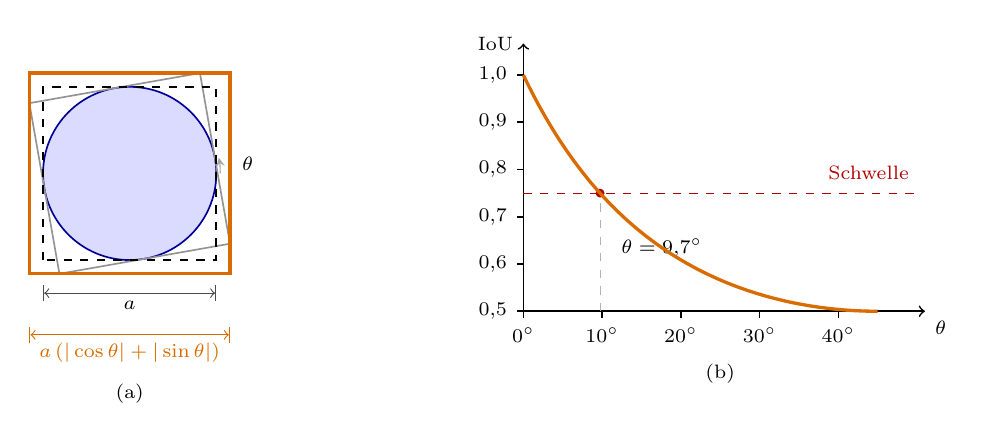
\begin{tikzpicture}
\begin{scope}
  \fill[blue!14] (0,0) circle (1.1);
  \draw[blue!60!black,semithick] (0,0) circle (1.1);
  \begin{scope}[rotate=10]
    \draw[gray!85,semithick] (-1.1,-1.1) rectangle (1.1,1.1);
  \end{scope}
  \draw[dashed,thick] (-1.1,-1.1) rectangle (1.1,1.1);
  \draw[very thick,orange!85!black] (-1.2744,-1.2744) rectangle (1.2744,1.2744);
  \draw[->,>=stealth,gray!70] (1.15,0) arc (0:10:1.15);
  \node[font=\scriptsize] at (1.50,0.12) {$\theta$};
  \draw[|<->|,gray!60!black,thin] (-1.1,-1.52) -- (1.1,-1.52);
  \node[font=\scriptsize,anchor=north] at (0,-1.50) {$a$};
  \draw[|<->|,orange!85!black,thin] (-1.2744,-2.05) -- (1.2744,-2.05);
  \node[font=\scriptsize,anchor=north,orange!85!black] at (0,-2.03)
       {$a\,(|\cos\theta| + |\sin\theta|)$};
  \node[font=\scriptsize,anchor=north] at (0,-2.55) {(a)};
\end{scope}
\begin{scope}[shift={(5.0,-1.75)}]
  \draw[->,semithick] (0,0) -- (5.1,0) node[below right,font=\scriptsize] {$\theta$};
  \draw[->,semithick] (0,0) -- (0,3.4) node[left,font=\scriptsize] {$\mathrm{IoU}$};
  \foreach \t in {0,10,20,30,40}
    \draw[semithick] ({\t*0.1},0) -- ({\t*0.1},-0.08)
          node[below,font=\scriptsize] {$\t^\circ$};
  \foreach \v/\l in {0/{0,5}, 0.6/{0,6}, 1.2/{0,7}, 1.8/{0,8}, 2.4/{0,9}, 3.0/{1,0}}
    \draw[semithick] (0,\v) -- (-0.08,\v) node[left,font=\scriptsize] {\l};
  \draw[dashed,red!70!black] (0,1.5) -- (5.0,1.5);
  \node[font=\scriptsize,red!70!black,anchor=south east] at (5.02,1.55)
        {Schwelle \mAPseven};
  \draw[dashed,gray!60] ({9.74*0.1},0) -- ({9.74*0.1},1.5);
  \fill[red!70!black] ({9.74*0.1},1.5) circle (1.6pt);
  \node[font=\scriptsize,anchor=west] at (1.12,0.80) {$\theta = 9{,}7^\circ$};
  \draw[very thick,orange!85!black,smooth]
    plot[domain=0:45,samples=91]
    ({\x*0.1}, {(1/(1+sin(2*\x)) - 0.5)*6});
  \node[font=\scriptsize,anchor=north] at (2.5,-0.55) {(b)};
\end{scope}
\end{tikzpicture}
\caption[Boxaufblähung unter Bildrotation]{Bildrotation als Quelle von
Labelrauschen. (a)~Ein rotationssymmetrisches Objekt behält unter Rotation
dieselbe korrekte Box (schwarz gestrichelt); die mitgedrehte Box (grau) und ihre
achsparallele Hülle (orange) sind jedoch größer. (b)~Verlauf nach
Gleichung~\eqref{eq:ioutheta}: Bei $2^\circ$ liegt die Überlappung noch bei
0,935, bei $10^\circ$ bereits bei 0,745 und bei $45^\circ$ bei 0,500.}
\label{abb:boxrotation}
\end{figure}

Für ein Objekt von 25\px{} Durchmesser wächst die Boxkantenlänge bei $10^\circ$
um rund 4\px{} -- systematisches Rauschen im Zielsignal der Boxregression
(Abbildung~\ref{abb:boxrotation}). Die Konsequenz: Bildrotation, Scherung und Perspektive dürfen \emph{nicht} als
bildweite Trainingszeit-Augmentierung eingesetzt werden, wenn dieselbe Variation
auch label-exakt erzeugt werden kann -- was ein Generator leistet, der die Box
nach der Transformation aus der transformierten Alphamaske neu bestimmt.

\subsection{Kleine Objekte, Auflösung und Labelzuweisung}
\label{sec:ioukleinobjekt}

Verschiebt man eine quadratische Box der Kantenlänge $d$ um $\delta$ Pixel in
einer Achse, so gilt
\begin{equation}
\mathrm{IoU} \;=\; \frac{(d-\delta)\,d}{2d^2 - (d-\delta)\,d}
\;=\; \frac{1 - \delta/d}{1 + \delta/d} .
\label{eq:ioushift}
\end{equation}
Der Fehler wirkt ausschließlich über das \emph{Verhältnis} $\delta/d$: Für ein
20\px-Objekt kostet ein Boxfehler von 2\px{} bereits 0,18 IoU, bei diagonaler
Verschiebung 0,32; für ein 200\px-Objekt wäre derselbe absolute Fehler mit 0,02
IoU unsichtbar. \mAPall{} ist bei dieser Objektgröße folglich mehr ein Maß für
die Pixelauflösung als für die Detektionsqualität.

\begin{figure}[htbp]
\centering
\begin{tikzpicture}
\begin{scope}
  \node[font=\scriptsize,anchor=west] at (-0.15,3.35)
       {\textcolor{black}{$-\,-$ Ground Truth}\quad
        \textcolor{orange!85!black}{$-\!-$ Vorhersage}};
  \fill[pattern=north east lines,pattern color=orange!45]
       (0.72,0) rectangle (2.4,2.4);
  \draw[dashed,thick] (0,0) rectangle (2.4,2.4);
  \draw[very thick,orange!85!black] (0.72,0) rectangle (3.12,2.4);
  \draw[|<->|,gray!60!black,thin] (0,2.66) -- (0.72,2.66)
        node[midway,above,font=\scriptsize,inner sep=1pt] {$\delta$};
  \draw[|<->|,gray!60!black,thin] (-0.28,0) -- (-0.28,2.4)
        node[midway,fill=white,inner sep=1pt,font=\scriptsize] {$d$};
  \node[font=\scriptsize,anchor=north] at (1.5,-0.25) {(a)};
\end{scope}
\begin{scope}[shift={(5.0,-0.35)}]
  \draw[->,semithick] (0,0) -- (4.7,0)
        node[below right,font=\scriptsize] {$\delta/d$};
  \draw[->,semithick] (0,0) -- (0,3.4) node[left,font=\scriptsize] {$\mathrm{IoU}$};
  \foreach \t/\l in {0.1/{0,1}, 0.2/{0,2}, 0.3/{0,3}, 0.4/{0,4}}
    \draw[semithick] ({\t*8},0) -- ({\t*8},-0.08)
          node[below,font=\scriptsize] {\l};
  \foreach \v/\l in {0.75/{0,25}, 1.5/{0,5}, 2.25/{0,75}, 3.0/{1,0}}
    \draw[semithick] (0,\v) -- (-0.08,\v) node[left,font=\scriptsize] {\l};
  \draw[dashed,red!70!black] (0,1.5) -- (4.6,1.5);
  \draw[dashed,red!30!black] (0,2.25) -- (4.6,2.25);
  \node[font=\scriptsize,red!30!black,anchor=north east,fill=white,
        inner sep=1pt] at (4.58,2.21) {Schwelle 0,75};
  \node[font=\scriptsize,red!70!black,anchor=south east,fill=white,
        inner sep=1pt] at (4.58,1.53) {Schwelle 0,50};
  \draw[very thick,orange!85!black,smooth]
    plot[domain=0:0.45,samples=60] ({\x*8}, {((1-\x)/(1+\x))*3});
  \draw[very thick,blue!60!black,densely dashed,smooth]
    plot[domain=0:0.45,samples=60]
    ({\x*8}, {(((1-\x)*(1-\x))/(2-(1-\x)*(1-\x)))*3});
  \node[font=\scriptsize,anchor=west,orange!85!black] at (3.68,1.14)
       {achsparallel};
  \node[font=\scriptsize,anchor=west,blue!60!black] at (3.68,0.53)
       {diagonal};
  \fill[orange!85!black] (0.8,{(0.9/1.1)*3}) circle (1.5pt);
  \fill[blue!60!black]   (0.8,{(0.81/1.19)*3}) circle (1.5pt);
  \node[font=\scriptsize,anchor=south west,fill=white,inner sep=1pt]
       at (0.90,{(0.9/1.1)*3}) {$\delta=2$\,px bei $d=20$\,px};
  \node[font=\scriptsize,anchor=north] at (2.3,-0.55) {(b)};
\end{scope}
\end{tikzpicture}
\caption[Empfindlichkeit der IoU gegenüber Boxversatz]{Empfindlichkeit der IoU
gegenüber einem Boxversatz. (a)~Zwei Boxen der Kantenlänge $d$, um $\delta$
verschoben; schraffiert der Schnitt. (b)~Verlauf nach
Gleichung~\eqref{eq:ioushift} für achsparallele und für diagonale Verschiebung.
Der Fehler wirkt allein über das Verhältnis $\delta/d$: Die Schwelle 0,75 wird
bei $\delta/d = 1/7$ unterschritten (2,9\px{} bei einem 20\px-Objekt), die
Schwelle 0,50 bei $\delta/d = 1/3$ (6,7\px).}
\label{abb:iouversatz}
\end{figure}

Detektoren verarbeiten Bilder in einer festen Netzeingangsgröße $M$
(\code{imgsz}); ein Bild mit längster Kante $N$ wird um $M/N$ skaliert. Ein
Objekt mit Durchmesser $d$ erreicht das Netz damit mit
\begin{equation}
d_{\text{eff}} \;=\; d \cdot \frac{M}{N} .
\label{eq:deff}
\end{equation}
Für $N = 2459$, $d = 27$\px{} und $M = 640$ ergibt das
$d_{\text{eff}} = 7{,}0$\px{} -- weniger als die Schrittweite $S = 8$ der
feinsten Standard-Detektionsebene. Wie folgenreich das ist, zeigt die Zahl der
Gitterzellen, deren Zentrum in das Objekt fällt und die damit bei einem
ankerfreien Kopf überhaupt als positive Zuweisung in Frage kommen. Für ein
kreisförmiges Objekt vom Durchmesser $d$ auf einer Ebene mit Schrittweite $S$
beträgt dieser Erwartungswert, gemittelt über die Lage des Objektzentrums im
Gitter,
\begin{equation}
\mathbb{E}[N_{\text{Zellen}}] \;=\; \frac{\pi d^2}{4 S^2} ,
\label{eq:zellen}
\end{equation}
und unterhalb von $d < S\sqrt{2} \approx 1{,}41\,S$ existieren Lagen, bei denen
\emph{kein} Zellzentrum im Objekt liegt -- das Objekt erhält dann keine positive
Zuweisung. Für $S = 8$ liegt diese Grenze bei 11,3\px, also genau im Bereich der
hier auftretenden Objektgrößen. Genau dieses Problem adressieren die
Small-Target-Aware Label Assignment von YOLO26 auf der Verlustseite und ein
zusätzlicher P2-Kopf auf der Architekturseite;
\textcite{kisantal2019} adressieren es auf der Datenseite durch Überabtastung
kleiner Objekte. Für die Augmentierung folgt daraus eine Randbedingung: Die
Größenverteilung der Trainingsobjekte und die effektive Größenverteilung zur
Inferenzzeit müssen übereinstimmen; eine Trainingsskalierung, die Objekte unter
$S$ schrumpfen lässt, erzeugt Labels ohne auflösbares Objekt.

\begin{figure}[htbp]
\centering
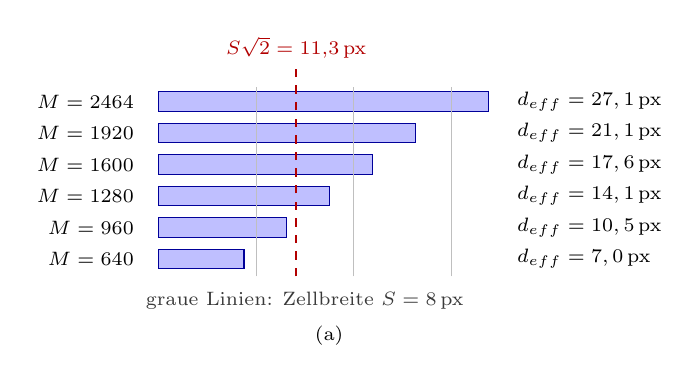
\begin{tikzpicture}[x=0.155cm,y=1cm]
  \foreach \m/\deff/\lab/\row in {%
      640/7.03/{7,0}/0, 960/10.54/{10,5}/1, 1280/14.05/{14,1}/2,
      1600/17.57/{17,6}/3, 1920/21.08/{21,1}/4, 2464/27.05/{27,1}/5}{
    \node[font=\scriptsize,anchor=east] at (-1.2,{\row*0.40}) {$M=\m$};
    \fill[blue!25] (0,{\row*0.40-0.125}) rectangle (\deff,{\row*0.40+0.125});
    \draw[blue!60!black,thin] (0,{\row*0.40-0.125}) rectangle (\deff,{\row*0.40+0.125});
    \node[font=\scriptsize,anchor=west] at (28.6,{\row*0.40})
         {$d_{\text{eff}} = \lab$\,px};
  }
  \foreach \k in {1,2,3}
    \draw[gray!50,very thin] ({\k*8},-0.22) -- ({\k*8},2.18);
  \draw[dashed,thick,red!70!black] (11.31,-0.22) -- (11.31,2.42);
  \node[font=\scriptsize,red!70!black,anchor=south] at (11.31,2.42)
       {$S\sqrt{2} = 11{,}3$\,px};
  \node[font=\scriptsize,gray!45!black,anchor=north] at (12,-0.30)
       {graue Linien: Zellbreite $S = 8$\,px};
  \node[font=\scriptsize,anchor=north] at (14,-0.72) {(a)};
\end{tikzpicture}

\vspace{5mm}
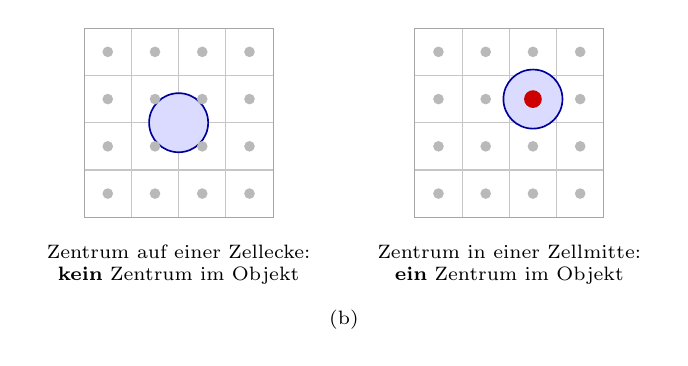
\begin{tikzpicture}[x=0.075cm,y=0.075cm]
\foreach \sh/\ox/\oy/\lab in {%
   0/16/16/{Zentrum auf einer Zellecke:\\\textbf{kein} Zentrum im Objekt},
   56/20/20/{Zentrum in einer Zellmitte:\\\textbf{ein} Zentrum im Objekt}}{
  \begin{scope}[shift={(\sh,0)}]
    \draw[step=8,gray!45,thin] (0,0) grid (32,32);
    \draw[gray!70] (0,0) rectangle (32,32);
    \fill[blue!14] (\ox,\oy) circle (5);
    \draw[blue!60!black,semithick] (\ox,\oy) circle (5);
    \foreach \i in {0,1,2,3}{\foreach \j in {0,1,2,3}{
      \pgfmathsetmacro{\cx}{4+8*\i}
      \pgfmathsetmacro{\cy}{4+8*\j}
      \pgfmathsetmacro{\dd}{sqrt((\cx-\ox)^2+(\cy-\oy)^2)}
      \ifdim\dd pt<5pt
        \fill[red!80!black] (\cx,\cy) circle (1.5);
      \else
        \fill[gray!55] (\cx,\cy) circle (0.9);
      \fi}}
    \node[font=\scriptsize,anchor=north,align=center,text width=3.6cm]
         at (16,-3) {\lab};
  \end{scope}}
\node[font=\scriptsize,anchor=north] at (44,-14) {(b)};
\end{tikzpicture}
\caption[Effektive Objektgröße und Zuweisungsgrenze]{(a)~Effektive Objektgröße
nach Gleichung~\eqref{eq:deff} für ein Objekt von 27\px{} im 2459\px{} breiten
\code{val}-Bild; graue Linien im Abstand der Zellbreite $S = 8$\px. Erst ab
\code{imgsz}~1280 liegt $d_{\text{eff}}$ über der Grenze $S\sqrt{2}$.
(b)~Warum diese Grenze gilt: Ein Objekt von 10\px{} Durchmesser (Radius 5\px),
dessen Zentrum auf einer Zellecke liegt, enthält \emph{kein} Zellzentrum -- der
Abstand von der Ecke zum nächsten Zentrum beträgt $S/\sqrt{2} = 5{,}7$\px. Um
eine halbe Zelle verschoben enthält dasselbe Objekt eines. Unterhalb von
$d = S\sqrt{2} = 11{,}3$\px{} hängt die Zuweisung damit von der Lage im Gitter
ab.}
\label{abb:aufloesung}
\end{figure}

\subsection{Mehrbildverfahren}

Mosaic \parencite{bochkovskiy2020} fügt vier Trainingsbilder zu einem zusammen:
Es erhöht die Objektzahl pro Iteration, bringt Objekte an Kachelränder und
kombiniert Hintergründe, wobei die Boxen exakt bleiben, da nur beschnitten und
verschoben wird. Kehrseite ist eine Bildstatistik, die es zur Inferenzzeit nie
gibt -- weshalb Mosaic üblicherweise in den letzten Epochen abgeschaltet wird
\parencite{ultralyticsdocs}. Für mixup und CutMix gilt das nicht in gleicher
Weise: Beide überlagern Bildinhalte bei erhaltenen Labels und erzeugen bei der
Detektion halbtransparente Geisterobjekte mit vollem Boxlabel; bei dicht
gepackten 20\px-Objekten wirkt der Labelkonflikt wie Rauschen.

\section{Rein synthetische Trainingsdaten}
\label{sec:augsynthese}

Wird die Augmentierung so weit getrieben, dass sie die Trainingsdaten nicht
erweitert, sondern erzeugt, entsteht synthetische Datengenerierung; einen
Überblick über das Feld gibt \textcite{nikolenko2021}. Die
\textbf{Copy-Paste-Synthese} setzt freigestellte Objekte in reale Hintergründe
ein; die Literatur ergibt zusammengenommen die Entwurfsregel
\emph{Grenzfläche und Skala sind kritisch, Kontext ist wichtig, globale
Bildästhetik ist nachrangig}: \textcite{dwibedi2017} identifizieren als
entscheidenden Faktor nicht die globale Plausibilität, sondern die lokale
Grenzflächenqualität, \textcite{georgakis2017} ergänzen maßstabsgerechtes
Einsetzen, \textcite{dvornik2018} den Kontext, und \textcite{ghiasi2021} zeigen,
dass selbst kontextfreies Copy-Paste ein starker Augmentierer ist, sofern
Skalenvariation vorhanden ist. Die \textbf{Domain Randomization}
\parencite{tobin2017,tremblay2018} verfolgt die gegenläufige Idee: Statt
Realismus wird so viel Variation erzeugt, dass die reale Welt als eine weitere
Variation erscheint; \textcite{prakash2019} verbinden beides zur
\emph{strukturierten} Randomisierung innerhalb physikalisch plausibler Grenzen,
und \textcite{hinterstoisser2018} zeigen, dass vortrainierte Merkmalsextraktoren
den Übergang erleichtern. Die hier verfolgte Pipeline liegt zwischen beiden
Linien: breite Randomisierung, aber ausschließlich innerhalb physikalisch
möglicher Konfigurationen, und Hintergründe aus der Zieldomäne selbst.

\absatz{Warum der Übergang misslingt, wenn er misslingt.} Der Nutzen hängt daran,
wie ähnlich die erzeugte Verteilung $D_S$ der Zielverteilung $D_T$ ist.
\textcite{bendavid2010} geben dafür die Schranke
\begin{equation}
\varepsilon_T(h) \;\leq\; \varepsilon_S(h)
\;+\; d_{\mathcal{H}\Delta\mathcal{H}}(D_S, D_T) \;+\; \lambda
\label{eq:bendavid}
\end{equation}
an, mit dem Quellfehler $\varepsilon_S$, einer Divergenz zwischen den
Eingabeverteilungen und dem Fehler $\lambda$ der besten gemeinsamen Hypothese.
Sie listet die Angriffspunkte des Pipelineentwurfs vollständig auf:
\emph{(i)} $\varepsilon_S$ klein halten -- also korrekt gelabelte synthetische
Daten erzeugen, weshalb die Sichtbarkeit exakt gerechnet wird;
\emph{(ii)} $d_{\mathcal{H}\Delta\mathcal{H}}$ klein halten -- Zweck aller
Kalibrierungen an Realmessungen und aller Maßnahmen zum Einbettungsrealismus.
Wichtig ist die Struktur dieses Terms: Die Divergenz wird über die
Hypothesenklasse gemessen, ein Unterschied, den ein CNN \emph{leicht} erkennen
kann -- eine achsparallele Naht, ein konstanter Farbversatz --, trägt daher weit
stärker bei als ein Unterschied ohne einfache Entscheidungsfunktion;
\emph{(iii)} $\lambda$ klein halten -- die \emph{Labeldefinition} muss in Quelle
und Ziel identisch sein, weshalb die Pipeline modale Boxen erzeugt und Labels
nach denselben Regeln verwirft wie die Handannotation.

\absatz{Was die Schranke praktisch leistet.} Von den vier Größen sind zwei
messbar: der Fehler auf synthetischen und der auf realen Daten. Umgestellt liefert
Gleichung~\eqref{eq:bendavid} damit
\begin{equation}
d_{\mathcal{H}\Delta\mathcal{H}}(D_S, D_T) + \lambda \;\geq\;
\varepsilon_T(h) - \varepsilon_S(h),
\label{eq:bendavid-diff}
\end{equation}
also eine \emph{untere} Schranke für die Summe der beiden \emph{un}messbaren
Terme -- und zwar aus zwei Zahlen, die jede Auswertung ohnehin ausgibt. Genau
diese Differenz wird in Abschnitt~\ref{sec:simtoreal} als Sim-to-Real-Abstand
berichtet und dort in die Schranke eingesetzt. Auf die Richtung ist zu achten:
Die Ungleichung nagelt die Summe nach \emph{unten} fest; dass die Divergenz
\emph{klein} ist, kann sie nicht belegen.

\subsection{Shortcut Learning als konkrete Fehlerquelle}
\label{sec:shortcut}

Punkt~(ii) ist die Hauptfehlerquelle. \textcite{geirhos2020} beschreiben unter
\emph{Shortcut Learning} das Phänomen, dass Netze bevorzugt jene Merkmale nutzen,
die auf den Trainingsdaten am einfachsten zum Ziel führen -- auch wenn diese mit
der Aufgabe nichts zu tun haben und außerhalb der Trainingsverteilung nicht
gelten; \textcite{torralba2011} zeigen, dass schon gewöhnliche Bilddatensätze an
solchen Merkmalen erkennbar sind. Bei eingeklebten Objekten sind die Abkürzungen
benennbar, und die Bildforensik untersucht genau diese Signaturen, um Montagen
nachzuweisen \parencite{farid2009}. Tabelle~\ref{tab:signaturen} liest diese
Signaturen als Katalog der zu schließenden Lücken.

\begin{table}[htbp]
\centering
\caption[Signaturen eingeklebter Objekte]{Die sechs Signaturen, an denen sich
eingeklebte Bildinhalte verraten, und die jeweilige Gegenmaßnahme der Pipeline.}
\label{tab:signaturen}
\footnotesize
\begin{tabularx}{\textwidth}{@{}L{0.035\textwidth}L{0.24\textwidth}XL{0.235\textwidth}@{}}
\toprule
 & \textbf{Signatur} & \textbf{Warum sie erkennbar ist} &
\textbf{Gegenmaßnahme} \\
\midrule
S1 & geometrische Naht &
Ein rechteckiger Ausschnitt hinterlässt eine achsparallele Kante -- für ein CNN
trivial detektierbar &
Freistellen mit weicher Alphamaske \\
S2 & Farb- und Helligkeitsversatz &
Objekt und Hintergrund stammen aus Aufnahmen mit unterschiedlichem
Weißabgleich; der konstante Versatz ist global gültig &
partieller Statistikangleich \parencite{reinhard2001,tsai2017} \\
S3 & Schärfe- und Auflösungsversatz &
Ein skaliertes Objekt hat eine andere Modulationsübertragung; Aliasing erzeugt
Hochfrequenzmuster \parencite{popescu2005,zhangr2019} &
flächentreue Verkleinerung, Unschärfeangleich \\
S4 & Rauschversatz &
Beim Verkleinern sinkt das Sensorrauschen -- der eingeklebte Bereich ist
messbar sauberer; Rauschen ist kameraspezifisch \parencite{lukas2006} &
Rauschangleich mit lokal geschätzter Amplitude \parencite{immerkaer1996} \\
S5 & Kompressionsversatz &
Der Hintergrund war bereits JPEG-komprimiert, die eingefügten Pixel nicht; die
DCT-Blockstatistik unterscheidet sich \parencite{wallace1992jpeg} &
erneute Requantisierung des \emph{Gesamtbildes} \\
S6 & fehlende Szeneninteraktion &
Ohne Kontaktschatten und plausible Verdeckung \enquote{schwebt} das Objekt
sichtbar &
Schlagschatten, physikalisch motivierte Verdeckung \\
\bottomrule
\end{tabularx}
\end{table}

Der entscheidende Punkt: Bei Copy-Paste-Synthese ist \emph{nicht zu wenig
Variation} die dominante Fehlerquelle, sondern der \emph{systematische}
Unterschied zwischen eingefügten und originalen Pixeln. Variation lässt sich
durch mehr Zufall erzeugen; ein systematischer Versatz bleibt bei beliebig viel
Zufall bestehen und wird vom Netz zuverlässig gefunden.

\section{Anforderungen an die Pipeline}
\label{sec:anforderungen}

\begin{description}[leftmargin=1.2em,itemsep=1pt,font=\normalfont\bfseries]
  \item[A1 -- Labelexaktheit] Jede Transformation muss eine exakt bekannte
  Labeltransformation besitzen; boxaufblähende Operationen sind bildweit verboten
  und pro Instanz mit Neuberechnung der Box auszuführen.
  \item[A2 -- Kalibrierte Skala] Die erzeugte Größenverteilung muss der
  gemessenen entsprechen, und die Objekte müssen oberhalb der Auflösungsgrenze
  der feinsten Detektionsebene liegen.
  \item[A3 -- Physikalische Zulässigkeit] Erzeugt werden nur real mögliche
  Konfigurationen; Invarianzen nur dort, wo sie gelten.
  \item[A4 -- Geschlossene Abkürzungen] Für jede Signatur S1--S6 muss eine
  Gegenmaßnahme existieren.
  \item[A5 -- Identische Labeldefinition] Die Regeln der Labelvergabe müssen mit
  denen der Handannotation übereinstimmen (Term $\lambda$).
  \item[A6 -- Dokumentierte Verteilung] Für jede Transformation sind
  Parameterbereich \emph{und} tatsächlicher Anteil anzugeben; Werte ohne
  Messbeleg sind als Annahme zu kennzeichnen.
\end{description}
